\parindent=1.5em

A través de los años el hombre ha presentado un cambio sustancial en su nivel
de vida; los conocimientos que ha logrado acumular y aplicar han sido para su
beneficio, y han cambiado radicalmente su modo de vivir. Existe una notable
diferencia entre el hombre de hace unas cuantas décadas y el hombre moderno.
Tal diferencia se ha dado por el desarrollo de la ciencia, que está
estrechamente relacionada con la innovación tecnológica. Por esta razón se
amplía el contenido de cómo ha evolucionado la ciencia y la tecnología en el
mundo, su origen remoto, los países que más han aportado en esta área y su
respectiva utilización, ya sea para el desarrollo o la destrucción. Como se
sabe, la tecnología se está haciendo presente en todas y cada una de las áreas
de investigación, como física, química, biología, computación, y lo que es de
interés para este documento es el área de los mercados financieros
\cite{watsham1997quantitative}.

Esta memoria está enfocada a abordar un problema relacionado con las series
financieras de alta frecuencia y una forma particular de poder realizar
pronósticos tomando en cuenta las distintas características de naturaleza
propia de este tipo de datos. Se pretende abordar esta problemática con
metodologías computacionales, aplicando algunos análisis matemáticos útiles
para esta área. El problema es de carácter financiero, por lo que es necesario
contextualizar el tema mediante conceptos, criterios y términos generales
asociados al área.

Este capítulo tiene como objetivo introducir los conceptos de series de tiempo
financieras, sus orígenes y la alta frecuencia.

\section{Mercados Financieros}

El mercado financiero es un espacio con marco institucional que permite poner
en contacto a oferentes y demandantes para que efectúen transacciones
financieras. La idea de mercado como foro organizado a la que acuden agentes
económicos para efectuar transacciones queda reducida en el mundo financiero
como las bolsas de valores \cite{mishkin2006financial}.

El concepto de mercado financiero se utiliza en general para referirse a
cualquier mercado organizado en el que se negocien instrumentos financieros de
todo tipo, como acciones, divisas, etc. El espacio para generar estas
interacciones no necesariamente debe ser físico. Por otro lado, el negociar
instrumentos financieros implica a grandes rasgos: definir su precio e
intercambiarlos, por ende, estos mercados están basados en las fuerzas de
oferta y demanda, ubicando a todos los oferentes en el mismo lugar, y así
facilitarle la búsqueda a los demandantes. Dentro de este tipo de mercado se
distinguieron bloques de estudio en la economía moderna
\cite{jensen1984theory}.

Una de las razones que hace importante este tipo de mercado, es su
funcionalidad, ya que permiten: por un lado aumentar el capital, siendo esto
uno de los casos favorables, ya que también hay probabilidades considerables de
disminuir el capital; comercio internacional, como en los mercados de divisas,
por ejemplo Forex; y reunir a quienes necesitan recursos financieros, con los
que tienen recursos financieros. Factores que permiten generar los efectos de
oferta y demanda.

En este tipo de mercado se definen los siguientes términos \cite{nevmyvaka2003electronic}:
\begin{itemize}
	\item \emph{Dealer}: Un dealer es un ente presente en los mercados que está
dispuestos a comprar o vender.
	\item \emph{Orders}: Operación de compra/venta de activos.
	\item \emph{Bid price}: Precio al cual un \emph{dealer} está dispuesto a
comprar.
	\item \emph{Ask price}: Precio al cual un \emph{dealer} está dispuesto a
vender.
	\item \emph{Market orders}: instrucción del cliente al dealer, de comprar o
vender al mejor precio posible dentro de los valores actuales del mercado.
Esto asegura la realización de la transacción, pero no el precio.
	\item \emph{Limit orders}: es una orden para comprar a un valor máximo
(precio determinado), o para vender a un valor mínimo (precio determinado).
Esto le da al cliente el control sobre el precio al que se ejecuta el comercio,
sin embargo, no garantiza la realización de la transacción.
\end{itemize}

El conjunto de \emph{Limit orders} forman los \emph{books} para cierto
instrumento, los cuales proveen información detallada del mismo. Con estos
datos se forman los llamados bid-ask spreads, que es la diferencia entre el
precios cotizados para una venta inmediata (oferta) y una compra inmediata
(bid).  También se generan los bid-ask qoute, el cual define cotas para el
precio de transacción.

\subsection{Mercados bursátiles}
Los mercados bursátiles están clasificados dentro de los mercados de capitales,
en donde se negocian activos financieros. Este tipo de mercado provee
financiamiento por medio de la emisión de acciones y permiten luego el
intercambio de estas. La aplicación más directa de este tipo de mercados, son
las bolsas de valores, cuyo origen se remonta a finales del siglo XV en las
ferias medievales de Europa. Las bolsas de valores se pueden definir como
mercados organizados y especializados, en los que se pueden realizar
transacciones de títulos de valores por medio de intermediarios autorizados.
Estas bolsas ofrecen al público y a sus miembros facilidades, mecanismos e
instrumentos técnicos que facilitan la negociación de títulos de valores
susceptibles de ofertas públicas, y precios determinados mediante subasta
\cite{levine1998stock}.

La principal función de las Bolsas de Valores es proporcionar a los
participantes información objetiva, completa y permanente de los valores y las
empresas inscritas en la bolsa, sus emisiones y las operaciones que en ella se
realicen. Además debeb supervisar las actividades. Las componentes de este
sistema son los activos y las instituciones financieras, cuya misión es
contactar demandantes y oferentes en los mercados donde se negocian los
diferentes instrumentos o activos financieros. En el documento se hablará de
instrumento, ya que pueden ser acciones, divisas, etc. los cuales quedan
generalizados bajo ese concepto.

La economía presenta a este tipo de mercado, como de competencia perfecta, ya
que sus características principales son: elevado número de compradores y
vendedores; La decisión individual de cada uno de ellos ejercerá escasa
influencia sobre el mercado global; Homogeneidad de los productos, es decir, no
existen diferencias entre productos que venden los oferentes; Transparencia del
mercado, todos los participantes tienen pleno conocimiento de las condiciones
generales en que opera el mercado; Libertad de entrada y salida de empresas,
todos los participantes, cuando lo deseen, podrán entrar o salir del mercado a
costos nulos o casi nulos \cite{mankiw2011principles}. 

Por otra parte, Fama propuso la Hipótesis de eficiencia de los mercados
\cite{malkiel2012efficient}, la cual establece que los mercados son eficientes
cuando son capaces de trasladar a los precios de los instrumentos financieros,
todos los datos relevantes, por lo tanto, el precio refleja \emph{toda} la
información disponible, y lo hace de manera insesgada. Cuando se cumplen estas
condiciones, el precio del instrumento financiero se comporta como un
\emph{Random Walk} \cite{fama1965random}, por lo que los resultados no pueden
ser predichos sistemáticamente.

\section{Series de tiempo financiera}

La mayoría de los fenómenos que se estudian en su componente temporal, deben
tomar en cuenta la dinámica de los proceso con la finalidad tener una
comprensión general del proceso. Una herramienta útil en dicho objetivo es el
análisis de series de tiempo. Una serie de tiempo, es una secuencia de datos
indexados por su marca temporal. Se pueden presentar casos de series de tiempo
en una multitud de disciplinas como ingeniería, sociología, economía, finanzas
por solo mencionar algunas de ellas.

El propósito fundamental es mostrar las técnicas que permitan hacer inferencias
del proceso en estudio incluyendo su predicción. Esto se logra estableciendo
modelos probabilísticos hipotéticos que representen a los datos; y en
consecuencia, se lleva a cabo el proceso de ajuste, que incluye desde la
estimación hasta la predicción, una vez que se ha determinado un modelo
satisfactorio para la muestra de datos \cite{box2011time}
\cite{vandaele1983applied}. Los modelos de series deben considerar la
naturaleza del fenómeno y determinar los factores que pueden ser incluidos en
el.

En particular, el análsis de una serie de tiempo financiera puede enfocarse en
analizar de forma teórica y práctica la valoración de cierto instrumento en el
tiempo, como también los volúmenes transados, etc. Lo que se intenta es modelar
la incertidumbre generada por las características propias de este fenómeno
\cite{tsay2005analysis}. 

Las características diferenciadoras han propiciado numerosos trabajos en las
áreas de econometría y economía financiera desde los años 60. Es por ello que,
en el área financiera las evidencias sobre patrones ha conducido a la
formulación de distintos modelos matemáticos.

\subsection{Descripción de serie financiera}

Una tendencia en el análisis de las series financieras, es el seguimiento del
precio de un instrumento en el tiempo.
%Las series de tiempo financieras, se basan en el estudio del precio de un
%instrumento financiero en el tiempo. 
Existen varios tipos de precios que se pueden analizar, por un lado están los
indicadores que se utilizaron en los primeros estudios formales, los cuales
mostraban información al respecto de los precios de: \emph{apertura},
\emph{cierre}, \emph{el más bajo}, \emph{el más alto}, \emph{promedio}. Esos
datos estaban orientados a tomar métricas respecto a valores que resumían los
cambios de precio de un instrumento en un día. Una muestra gráfica de esta
información sería la siguiente:
%con estos datos quedaban gráficos como el siguiente:

\begin{center}
	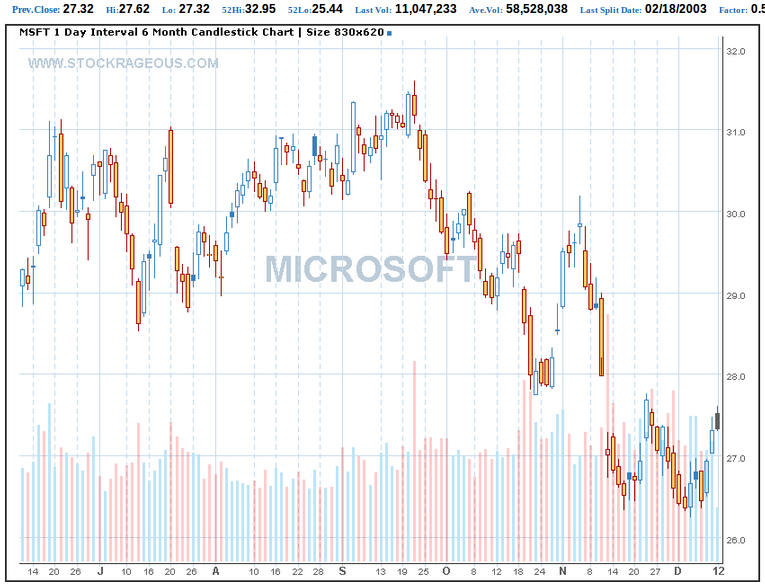
\includegraphics[width=0.8\textwidth]{images/microsoft} \\
	\textbf{Figura 1.} Información de los precios de microsoft en la bolsa.
Tomada desde \url{http://www.stockrageous.com/}.
\end{center}

Con esa información se realizaban \emph{estudios técnicos}
\cite{taylor1992use}, los cuales proporcionaban pronósticos de tendencias (como
subir o bajar de precio), basándose en la inspección visual y búsqueda de
patrones en los precios anteriores del instrumento. 

Sin embargo la data estudiada actualmente corresponde a data \emph{intra
diaria}, la cual reside en los valores específicos en que se compró o vendió
algún instrumento.  Ese precio se conoce como el \emph{last price}, y
corresponde al valor específico con el cual se realizó la transacción. La forma
de como se efecúa este evento es mediante los \emph{market} o \emph{limit
orders}, donde existe una cola de compras o ventas obtenidas mediante los
\emph{limit orders} y que cuando se cumpla la condición asociada (de vender o
comprar a cierto precio), se realiza la transacción y se registra dicho
\emph{last price}; por otro lado, si se entra a comprar/vender directamente
mediante una \emph{market order} también se registra dicho valor. Recopilando
esa información, se puede generar una secuencia temporal de los \emph{last
prices}. Estudios prácticos de estas series \cite{biais2012empirical},
generalizan su gráfica con forma de \emph{U},

A través de la historia, estas interacciones se realizaban personalmente en las
bolsas de comercio, en los llamados \emph{floor market}
\cite{jain2005financial}, sin embargo con el avance de las tecnologías, se han
implementado distintas plataformas de \emph{trading electrónico}: un método de
negociación de instrumentos financieros por medios electrónicos
\cite{weston2002electronic}. Estas tecnologías se utilizan para reunir a
compradores y vendedores a través de plataformas de comercio electrónico, como
por ejemplo: National Association of Securities Dealers Automated Quotation
(NASDAQ), New York Stock Exchange (NYSE), etc. Tomando en cuenta las nuevas
frecuencias de aparición de datos, en el orden de fracción de segundos, se
torna difícil manejar los datos de forma humana, es por esta razón que es
necesario realizar análisis cuantitativos mediante algoritmos computacionales.

Las series financieras de alta frecuencia tienen características particulares
en relación a otras series, como son: 
\begin{itemize}
	\item Frecuencia: la frecuencia en la observación de los datos es mayor que
en otro tipo de series de tiempo, en el orden de fracción de segundos.
	\item Heterocedasticidad: ocurre cuando la varianza de las perturbaciones
no es constante a lo largo de las observaciones.  Este factor hace inadecuados
los modelos desarrollados para series estacionarias.
	\item No estacionalidad: en muchos casos la media y varianza se presentan
como no estacionarias.
	\item Información oculta: se pueden encontrar distintos tipos de patrones a
diferentes niveles de escala.
\end{itemize}

\subsection{High frequency trading}

Con el paso del tiempo y la implementación de distintos sistemas de trading
electrónico, la frecuencia de la data aumentó, pasando de minutos a fracciones
de segundos.  En estos sistemas se define como unidad atómica de información un
\emph{Tick}. Un \emph{Tick} especifica una gran cantidad de parámetros como la
marca temporal, precio, cantidad transada, etc.  Los datos de alta frecuencia
son un conjunto de datos de reportes detallados sobre la actividad y movimiento
efectuados sobre un instrumento. Se reúne la información de los ticks con
cierto intervalo de tiempo, el cual para este tipo de series es variable. En la
literatura se puede encontrar más de un término para definir este fenómeno
\cite{ei2007quantitative}, como (ultra-)high-frequency data, microstructure
data, entre otros.

Los sistemas informáticos que realizan la labor de facilitar el comercio de
instrumentos financieros, son los llamados \emph{Electronic communication
networks} (ECN).  Se crearon en 1998, año que fueron autorizados por la
\emph{Securities and Exchange Commission}. La SEC \cite{hasbrouck2004economic}
es una organización estadounidense creada en 1933, y tiene la responsabilidad
de velar por el cumplimiento de las leyes federales las bolsas de valores. Un
caso emblemático, fue el 6 de mayo del 2010, fecha en la cual ocurrió el
\emph{Flash-Crash} \cite{arndt2011high}, dio a lugar a una quiebra financiera
estadounidense en el que el índice Dow Jones Industrial Average se desplomó un
9\%.

\section{High Performance Computing}

La capacidad de cómputo de los procesadores actuales ha incrementado, al igual
que la cantidad de procesadores de las CPU y también las que tienen las
tarjetas de video. Además, la naturaleza de los problemas que se están
estudiando tales como: simulación de tsunami, series de tiempo financiera,
entre otros; al crear modelos más realistas, es decir, que tomen en cuenta una
mayor cantidad de características del fenómeno, se van generando grandes
cantidades de cómputos, por lo que es necesario optimizar y hacer más
eficientes los algoritmos. Es por esto que nace el concepto de HPC, una forma
de aprovechar los recursos computacionales actuales, tanto en hardware como
software. El objetivo es poder a realizar eficientemente tareas que implican
alta cantidad de cómputos o que requieren manejo de grandes volúmenes de
información. 

\subsection{Graphics Processing Unit}
%CUDA
Las siglas GPU provienen de Graphics Processing Unit, o en español Unidad de
procesamiento gráfico. Para efectos de hardware, la GPU funciona como
coprocesador, pudiéndose utilizar de forma simultánea a la CPU y así aprovechar
el potencial que puedan ofrecer ambas al mismo tiempo.  Una GPU era un
procesador diseñado para llevar a cabo cálculos necesarios en la generación de
gráficos, sin embargo, actualmente tienen una componente multipropósito,
pudiendose realizar distintos tipos de operaciones. Hoy en día las GPU son más
potentes y pueden incluso superar frecuencias de reloj de una CPU antigua, pero
un factor importante, es que poseen una arquitectura que permite el paralelismo
masivo.

Una GPU está formada por cientos de pequeños núcleos que trabajan juntos para
procesar los datos de alguna aplicación. Esta arquitectura de procesamiento
paralelo masivo es la que proporciona al GPU su alta capacidad de cálculo.
Existen numerosas aplicaciones aceleradas en la GPU que brindan una forma
rápida de acceder a la computación de alto desempeño (High Performance
Computing). Durante los últimos años se han desarrollado nuevas tecnologías y
arquitecturas que permiten obtener mayor provecho a sus capacidades
\cite{owens2007gpu}.

El concepto implícito en todo este tema es el paralelismo, que es una forma de
computación en la cual varios cálculos pueden realizarse simultáneamente,
siempre y cuando no existan dependencias secuenciales entre ellos. Un ejemplo
es el "divide y vencerás", principio que busca dividir los problemas grandes,
en varios problemas pequeños, que son posteriormente solucionados en paralelo.

La evolución de las tarjetas gráficas ha venido acompañado de un gran
crecimiento en el mundo de los videojuegos y las aplicaciones 3D, realizándose
grandes producciones de chips gráficos por parte de grandes fabricantes, como
NVIDIA, AMD (ex ATI). Los recientes desarrollos sobre GPU abarcan distintas
áreas de la ciencia \cite{kirk2010programming}, como problemas astrofísicos
(n-body simulation), modelamiento molecular, computación financiera, etc. En
los últimos años también han aparecido conjuntos de herramientas y compiladores
que facilitan la programación de las GPUs, como por ejemplo, NVIDIA CUDA, que
cuenta con la comunidad más activa hasta la fecha en programación de GPUs.

\section{Motivación}

Dadas las características particulares que presentan las series financieras de
alta frecuencia, su análisis se puede transformar en una tarea árdua. La
literatura presenta distintos modelos y métodos para resolver este problema,
sin embargo no existe un método único que pueda solucionar este tipo problema.
Los métodos actuales inclusive, no consideran todas las características propias
de este tipo de fenómeno. La no existencia de un método que solucione este tipo
de problema, ha generado una tendencia de fusionar métodos, con el objetivo de
abodar de mejor forma el problema.

La mayor parte de los métodos, analizan este tipo de fenómenos en el dominio
del tiempo, lo que no ha presentado buenos resultados.  Uno de los enfoques, es
realizar análisis de Multiresolución Wavelet (MRA) \cite{benaouda2006wavelet},
centrando el estudio en el dominio de la frecuencia.  Este enfoque se ha
utilizado en distintas áreas de la ciencia, y en particular en series
financieras, teniendo resultados alentadores. Más en particular, Zhang ha
propuesto un modelo neural-wavelet \cite{zhang2001adaptive}, mezclando redes
neuronales con MRA, los cuales llegan a buenas aproximaciones pero no logran
competir en eficiencia temporal. La idea es poder rescatar información de la
serie por bandas, para luego realizar pronósticos (por bandas) mediante redes
neurnales, y se espera, que la predicción de multiple escala tenga mejor
performance de pronóstico que solamente una red. 

La motivación principal de esta memoria, es que el modelo no ha sido aplicado
para serie financieras de alta frecuencia, y en los casos que se ha
implementado, si bien ha tenido buenos resultados, no ha logrado tener buen
rendimiento a nivel de eficiencia, ya que el proceso involucra una alta
cantidad de cálculos. En base a esto se identificaron los objetivos para esta
memoria.

Los \emph{\textbf{objetivos principales}} son:
\begin{itemize}
	\item Implementar un modelo Neural-Wavelet y analizar su comportamiento con
series financieras de alta frecuencia.
	\item Optimizar dichos algoritmos usando computación heterogénea (CPU +
GPU) para aumentar su rendimiento.
\end{itemize} 

Los \emph{\textbf{objetivos secundarios}}:
\begin{itemize}
	\item Adaptar el modelo Neural-Wavelet para este tipo serie, encontrando
los parámetros apropiados para su funcionamiento.
	\item Encontrar una combinación de carga para CPU y GPU que permita hacer
más eficiente los cálculos.
\end{itemize}

\section{Organización de la Memoria}

Esta memoria se organizará con el siguiente esquema:
\begin{itemize}
	\item Capítulo 2: Estado del arte: se estudiarán y repasarán las técnicas
relativas a .
	\item Capítulo 3: Descripción formal del problema: se formalizará el
problema a resolver, indicando las características consideradas.
	\item Capítulo 4: Solución propuesta: se definirá una propuesta de
solución, con la respectiva metodología de implementación. 
	\item Capítulo 5: Estudio experimental: se implementará y testeará la
solución propuesta, comparando sus resultados.
	\item Capítulo 6: Conclusiones: se realizarán conclusiones generales del
trabajo realizado y se detallarán posibles trabajos futuros.
\end{itemize}
